\section{Halbtontechnik}

\subsection{Verfahren der Halbtontechnik}

\textit{
    Da nur Schwarz und Weiss gedruckt werden kann, werden
    die verschiedenen Stufen durch Intänsitätsstufen
    dargestellt. Dafür gibt es drei Verfahren:
}

\begin{itemize}
    \item Quantisierung
    \item Dithering
    \item Error Diffusion
\end{itemize}

\subsection{Quantisierung}

\textit{
    Höhere Auflösung auf tiefere Auflösung durch Runden
    der Pixelfarbwerte.
    Bsp. 16Bit -> 8Bit (Runden der Werte)
}

\subsection{Dithering}

\textit{
    Wenn der Drucker eine grössere Auflösung besitzt,
    jedoch weniger Farbstufen kann Dithering verfahren
    verwendet werden.
} \\

\subsection{Dithermatrizen}

\textit{
    Kann als Matrix dargestellt werden. Matrix gibt an,
    auf welcher stufe welche Pixel gesetzt werden
}

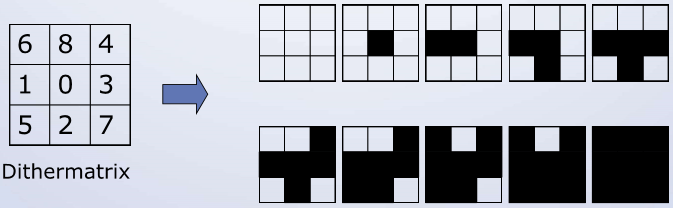
\includegraphics[width=0.45\textwidth]{assets/dithermatrix.png}

\textit{
    Es gibt zwei Regeln; Gesetzter \textbf{Pixel bleibt gesetzt} und \textbf{Strukturen}
    in der Ditheringmatrix \textbf{vermeiden}. Es soll möglichst ein Kreis
    approximiert werden.
}

\subsection{Dithering bei gleich bleibender Auflösung}

\textit{Handhabung, wenn die Auflösung gleichbleibt}

\begin{itemize}
    \item Mittelwert von n x n Region mit Ditheringmatrix ersetzen.
    \item Dispersed Dot Dithering
\end{itemize}

\subsection{Dispersed Dot Dithering}

\textit{
    Bayer Matrizen können hierfür verwendet werden,
    wodurch die Methode Bayer Dithering genannt wird.
} \\

\begin{tabular}{cc}
    \textit{2 x 2 Bayer Matrix} & \textit{4 x 4 Bayer Matrix} \\
    \begin{tabular}{|c|c|}
        \hline
        0 & 2 \\
        \hline
        3 & 1 \\
        \hline
    \end{tabular} &
    \begin{tabular}{|c|c|c|c|}
        \hline
        0 & 8 & 2 & 10 \\
        \hline
        12 & 4 & 14 & 6 \\
        \hline
        3 & 11 & 1 & 9 \\
        \hline
        15 & 7 & 13 & 5 \\
        \hline
    \end{tabular}
\end{tabular} \\

$k =  \frac{W_{max}}{n*n+1}$ \\

\textit{$W_{max}$: Maximalwert des Pixels (255 bei 8Bit)} \\
\textit{$n$: Grösse der Matrix (2 x 2 => $n = 2$)} \\
\textit{$k$: Faktor für Umrechnung} \\

$I_{new} = \frac{I_{old}}{k}$ \\
\textit{
    Für jeden Pixel den neuen Wert ausrechnen,
    danach mit Bayermatrix den Wert vergleichen.
    Pixel setzen wenn $I(x,y)_{new} > D_{ij}$)
} \\

$i = x$ modulo $n$ \\
$j = y$ modulo $n$ \\

\subsection{Error Diffusion}

\textit{
    Anstatt Kreise, Punkte verschiedener Dichte anordnen.
    Das Bild wird dabei sequenziell durchlaufen; links -> rechts, oben -> unten
} \\
\textit{Error Diffusion verteilt den Fehler auf die umliegenden Pixel} \\

\begin{tabular}{|c|c|c|}
    \hline
    & & 7/16 \\
    \hline
    1/16 & 5/16 & 3/16 \\
    \hline
\end{tabular}

\textit{Gewichtungsmatrix}

\textit{Beispiel:}

\begin{tabular}{|c|c|c|c|}
    \hline
    X & 191 & 140 & 113 \\
    \hline
    244 & 221 & 105 & 100 \\
    \hline
\end{tabular} \\

\textit{$191 - 255 = -64$, da Pixel Schwarz (255), Fehler: $-64$}

\begin{tabular}{|c|c|c|c|}
    \hline
    X & X & 140 + (7/16 * -64) & 113 \\
    \hline
    244 + & 221 + & 105 + & 100 \\
    (1/16 * -64) & (5/16 * -64) & (3/16 * -64) & \\
    \hline
\end{tabular} \\

\textit{Wenn Wert > 128 = 255, ansonten Wert <= 128 = 0}